\section{RISC-V CPU Design Specification} \label{sec:spec}
\subsection{RISC-V 151 ISA}
Table \ref{tab:ISA} contains all of the instructions your processor is responsible for supporting.
It contains most of the instructions specified in the RV32I Base Instruction set, and allows us to maintain a relatively simple design while still being able to have a C compiler and write interesting programs to run on the processor.
For the specific details of each instruction, refer to sections 2.2 through 2.6 in the \href{https://github.com/riscv/riscv-isa-manual/releases/download/Ratified-IMAFDQC/riscv-spec-20191213.pdf}{RISC-V Instruction Set Manual}.

\subsubsection{CSR Instructions}
You will have to implement 2 CSR instructions to support running the standard RISC-V ISA test suite.
A CSR (or control status register) is some state that is stored independent of the register file and the memory.
While there are $2^{12}$ possible CSR addresses, you will only use one of them (\verb|tohost = 12'h51E|).
That means you only need to instantiate one 32-bit register.
The \texttt{tohost} register is monitored by the testbench, and simulation ends when a non-zero value is written to this register.
A CSR value of 1 indicates success, and a value greater than 1 indicates which test failed.

There are 2 CSR related instructions that you will need to implement:
\begin{enumerate}
  \item \verb|csrw tohost,x2|  (short for \verb|csrrw x0,csr,rs1| where \verb|csr = 12'h51E|)
  \item \verb|csrwi tohost,1|  (short for \verb|csrrwi x0,csr,uimm| where \verb|csr = 12'h51E|)
\end{enumerate}

\verb|csrw| will write the value from \verb|rs1| into the addressed CSR.
\verb|csrwi| will write the immediate (stored in the rs1 field in the instruction) into the addressed CSR.
Note that you do not need to write to \verb|rd| (writing to x0 does nothing).

\begin{table}[p]
  \caption{RISC-V ISA}
  \label{tab:ISA}
  \begin{small}
    \begin{center}
      \begin{tabular}{p{0in}p{0.4in}p{0.05in}p{0.05in}p{0.05in}p{0.05in}p{0.4in}p{0.6in}p{0.4in}p{0.6in}p{0.7in}l}
        & & & & & & & & & & \\
        &
        \multicolumn{1}{l}{\instbit{31}} &
        \multicolumn{1}{r}{\instbit{27}} &
        \instbit{26} &
        \instbit{25} &
        \multicolumn{1}{l}{\instbit{24}} &
        \multicolumn{1}{r}{\instbit{20}} &
        \instbitrange{19}{15} &
        \instbitrange{14}{12} &
        \instbitrange{11}{7} &
        \instbitrange{6}{0} \\
        \cline{2-11}


        &
        \multicolumn{4}{|c|}{funct7} &
        \multicolumn{2}{c|}{rs2} &
        \multicolumn{1}{c|}{rs1} &
        \multicolumn{1}{c|}{funct3} &
        \multicolumn{1}{c|}{rd} &
        \multicolumn{1}{c|}{opcode} & R-type \\
        \cline{2-11}


        &
        \multicolumn{6}{|c|}{imm[11:0]} &
        \multicolumn{1}{c|}{rs1} &
        \multicolumn{1}{c|}{funct3} &
        \multicolumn{1}{c|}{rd} &
        \multicolumn{1}{c|}{opcode} & I-type \\
        \cline{2-11}


        &
        \multicolumn{4}{|c|}{imm[11:5]} &
        \multicolumn{2}{c|}{rs2} &
        \multicolumn{1}{c|}{rs1} &
        \multicolumn{1}{c|}{funct3} &
        \multicolumn{1}{c|}{imm[4:0]} &
        \multicolumn{1}{c|}{opcode} & S-type \\
        \cline{2-11}


        &
        \multicolumn{4}{|c|}{imm[12$\vert$10:5]} &
        \multicolumn{2}{c|}{rs2} &
        \multicolumn{1}{c|}{rs1} &
        \multicolumn{1}{c|}{funct3} &
        \multicolumn{1}{c|}{imm[4:1$\vert$11]} &
        \multicolumn{1}{c|}{opcode} & B-type \\
        \cline{2-11}


        &
        \multicolumn{8}{|c|}{imm[31:12]} &
        \multicolumn{1}{c|}{rd} &
        \multicolumn{1}{c|}{opcode} & U-type \\
        \cline{2-11}


        &
        \multicolumn{8}{|c|}{imm[20$\vert$10:1$\vert$11$\vert$19:12]} &
        \multicolumn{1}{c|}{rd} &
        \multicolumn{1}{c|}{opcode} & J-type \\
        \cline{2-11}


        &
        \multicolumn{10}{c}{} & \\
        &
        \multicolumn{10}{c}{\bf RV32I Base Instruction Set} & \\
        \cline{2-11}


        &
        \multicolumn{8}{|c|}{imm[31:12]} &
        \multicolumn{1}{c|}{rd} &
        \multicolumn{1}{c|}{0110111} & LUI \\
        \cline{2-11}


        &
        \multicolumn{8}{|c|}{imm[31:12]} &
        \multicolumn{1}{c|}{rd} &
        \multicolumn{1}{c|}{0010111} & AUIPC \\
        \cline{2-11}


        &
        \multicolumn{8}{|c|}{imm[20$\vert$10:1$\vert$11$\vert$19:12]} &
        \multicolumn{1}{c|}{rd} &
        \multicolumn{1}{c|}{1101111} & JAL \\
        \cline{2-11}


        &
        \multicolumn{6}{|c|}{imm[11:0]} &
        \multicolumn{1}{c|}{rs1} &
        \multicolumn{1}{c|}{000} &
        \multicolumn{1}{c|}{rd} &
        \multicolumn{1}{c|}{1100111} & JALR \\
        \cline{2-11}


        &
        \multicolumn{4}{|c|}{imm[12$\vert$10:5]} &
        \multicolumn{2}{c|}{rs2} &
        \multicolumn{1}{c|}{rs1} &
        \multicolumn{1}{c|}{000} &
        \multicolumn{1}{c|}{imm[4:1$\vert$11]} &
        \multicolumn{1}{c|}{1100011} & BEQ \\
        \cline{2-11}


        &
        \multicolumn{4}{|c|}{imm[12$\vert$10:5]} &
        \multicolumn{2}{c|}{rs2} &
        \multicolumn{1}{c|}{rs1} &
        \multicolumn{1}{c|}{001} &
        \multicolumn{1}{c|}{imm[4:1$\vert$11]} &
        \multicolumn{1}{c|}{1100011} & BNE \\
        \cline{2-11}


        &
        \multicolumn{4}{|c|}{imm[12$\vert$10:5]} &
        \multicolumn{2}{c|}{rs2} &
        \multicolumn{1}{c|}{rs1} &
        \multicolumn{1}{c|}{100} &
        \multicolumn{1}{c|}{imm[4:1$\vert$11]} &
        \multicolumn{1}{c|}{1100011} & BLT \\
        \cline{2-11}


        &
        \multicolumn{4}{|c|}{imm[12$\vert$10:5]} &
        \multicolumn{2}{c|}{rs2} &
        \multicolumn{1}{c|}{rs1} &
        \multicolumn{1}{c|}{101} &
        \multicolumn{1}{c|}{imm[4:1$\vert$11]} &
        \multicolumn{1}{c|}{1100011} & BGE \\
        \cline{2-11}


        &
        \multicolumn{4}{|c|}{imm[12$\vert$10:5]} &
        \multicolumn{2}{c|}{rs2} &
        \multicolumn{1}{c|}{rs1} &
        \multicolumn{1}{c|}{110} &
        \multicolumn{1}{c|}{imm[4:1$\vert$11]} &
        \multicolumn{1}{c|}{1100011} & BLTU \\
        \cline{2-11}


        &
        \multicolumn{4}{|c|}{imm[12$\vert$10:5]} &
        \multicolumn{2}{c|}{rs2} &
        \multicolumn{1}{c|}{rs1} &
        \multicolumn{1}{c|}{111} &
        \multicolumn{1}{c|}{imm[4:1$\vert$11]} &
        \multicolumn{1}{c|}{1100011} & BGEU \\
        \cline{2-11}


        &
        \multicolumn{6}{|c|}{imm[11:0]} &
        \multicolumn{1}{c|}{rs1} &
        \multicolumn{1}{c|}{000} &
        \multicolumn{1}{c|}{rd} &
        \multicolumn{1}{c|}{0000011} & LB \\
        \cline{2-11}


        &
        \multicolumn{6}{|c|}{imm[11:0]} &
        \multicolumn{1}{c|}{rs1} &
        \multicolumn{1}{c|}{001} &
        \multicolumn{1}{c|}{rd} &
        \multicolumn{1}{c|}{0000011} & LH \\
        \cline{2-11}


        &
        \multicolumn{6}{|c|}{imm[11:0]} &
        \multicolumn{1}{c|}{rs1} &
        \multicolumn{1}{c|}{010} &
        \multicolumn{1}{c|}{rd} &
        \multicolumn{1}{c|}{0000011} & LW \\
        \cline{2-11}


        &
        \multicolumn{6}{|c|}{imm[11:0]} &
        \multicolumn{1}{c|}{rs1} &
        \multicolumn{1}{c|}{100} &
        \multicolumn{1}{c|}{rd} &
        \multicolumn{1}{c|}{0000011} & LBU \\
        \cline{2-11}


        &
        \multicolumn{6}{|c|}{imm[11:0]} &
        \multicolumn{1}{c|}{rs1} &
        \multicolumn{1}{c|}{101} &
        \multicolumn{1}{c|}{rd} &
        \multicolumn{1}{c|}{0000011} & LHU \\
        \cline{2-11}


        &
        \multicolumn{4}{|c|}{imm[11:5]} &
        \multicolumn{2}{c|}{rs2} &
        \multicolumn{1}{c|}{rs1} &
        \multicolumn{1}{c|}{000} &
        \multicolumn{1}{c|}{imm[4:0]} &
        \multicolumn{1}{c|}{0100011} & SB \\
        \cline{2-11}


        &
        \multicolumn{4}{|c|}{imm[11:5]} &
        \multicolumn{2}{c|}{rs2} &
        \multicolumn{1}{c|}{rs1} &
        \multicolumn{1}{c|}{001} &
        \multicolumn{1}{c|}{imm[4:0]} &
        \multicolumn{1}{c|}{0100011} & SH \\
        \cline{2-11}

        &
        \multicolumn{4}{|c|}{imm[11:5]} &
        \multicolumn{2}{c|}{rs2} &
        \multicolumn{1}{c|}{rs1} &
        \multicolumn{1}{c|}{010} &
        \multicolumn{1}{c|}{imm[4:0]} &
        \multicolumn{1}{c|}{0100011} & SW \\
        \cline{2-11}

        &
        \multicolumn{6}{|c|}{imm[11:0]} &
        \multicolumn{1}{c|}{rs1} &
        \multicolumn{1}{c|}{000} &
        \multicolumn{1}{c|}{rd} &
        \multicolumn{1}{c|}{0010011} & ADDI \\
        \cline{2-11}

        &
        \multicolumn{6}{|c|}{imm[11:0]} &
        \multicolumn{1}{c|}{rs1} &
        \multicolumn{1}{c|}{010} &
        \multicolumn{1}{c|}{rd} &
        \multicolumn{1}{c|}{0010011} & SLTI \\
        \cline{2-11}

        &
        \multicolumn{6}{|c|}{imm[11:0]} &
        \multicolumn{1}{c|}{rs1} &
        \multicolumn{1}{c|}{011} &
        \multicolumn{1}{c|}{rd} &
        \multicolumn{1}{c|}{0010011} & SLTIU \\
        \cline{2-11}

        &
        \multicolumn{6}{|c|}{imm[11:0]} &
        \multicolumn{1}{c|}{rs1} &
        \multicolumn{1}{c|}{100} &
        \multicolumn{1}{c|}{rd} &
        \multicolumn{1}{c|}{0010011} & XORI \\
        \cline{2-11}

        &
        \multicolumn{6}{|c|}{imm[11:0]} &
        \multicolumn{1}{c|}{rs1} &
        \multicolumn{1}{c|}{110} &
        \multicolumn{1}{c|}{rd} &
        \multicolumn{1}{c|}{0010011} & ORI \\
        \cline{2-11}

        &
        \multicolumn{6}{|c|}{imm[11:0]} &
        \multicolumn{1}{c|}{rs1} &
        \multicolumn{1}{c|}{111} &
        \multicolumn{1}{c|}{rd} &
        \multicolumn{1}{c|}{0010011} & ANDI \\
        \cline{2-11}

        &
        \multicolumn{4}{|c|}{0000000} &
        \multicolumn{2}{c|}{shamt} &
        \multicolumn{1}{c|}{rs1} &
        \multicolumn{1}{c|}{001} &
        \multicolumn{1}{c|}{rd} &
        \multicolumn{1}{c|}{0010011} & SLLI \\
        \cline{2-11}

        &
        \multicolumn{4}{|c|}{0000000} &
        \multicolumn{2}{c|}{shamt} &
        \multicolumn{1}{c|}{rs1} &
        \multicolumn{1}{c|}{101} &
        \multicolumn{1}{c|}{rd} &
        \multicolumn{1}{c|}{0010011} & SRLI \\
        \cline{2-11}

        &
        \multicolumn{4}{|c|}{0100000} &
        \multicolumn{2}{c|}{shamt} &
        \multicolumn{1}{c|}{rs1} &
        \multicolumn{1}{c|}{101} &
        \multicolumn{1}{c|}{rd} &
        \multicolumn{1}{c|}{0010011} & SRAI \\
        \cline{2-11}

        &
        \multicolumn{4}{|c|}{0000000} &
        \multicolumn{2}{c|}{rs2} &
        \multicolumn{1}{c|}{rs1} &
        \multicolumn{1}{c|}{000} &
        \multicolumn{1}{c|}{rd} &
        \multicolumn{1}{c|}{0110011} & ADD \\
        \cline{2-11}

        &
        \multicolumn{4}{|c|}{0100000} &
        \multicolumn{2}{c|}{rs2} &
        \multicolumn{1}{c|}{rs1} &
        \multicolumn{1}{c|}{000} &
        \multicolumn{1}{c|}{rd} &
        \multicolumn{1}{c|}{0110011} & SUB \\
        \cline{2-11}

        &
        \multicolumn{4}{|c|}{0000000} &
        \multicolumn{2}{c|}{rs2} &
        \multicolumn{1}{c|}{rs1} &
        \multicolumn{1}{c|}{001} &
        \multicolumn{1}{c|}{rd} &
        \multicolumn{1}{c|}{0110011} & SLL \\
        \cline{2-11}

        &
        \multicolumn{4}{|c|}{0000000} &
        \multicolumn{2}{c|}{rs2} &
        \multicolumn{1}{c|}{rs1} &
        \multicolumn{1}{c|}{010} &
        \multicolumn{1}{c|}{rd} &
        \multicolumn{1}{c|}{0110011} & SLT \\
        \cline{2-11}

        &
        \multicolumn{4}{|c|}{0000000} &
        \multicolumn{2}{c|}{rs2} &
        \multicolumn{1}{c|}{rs1} &
        \multicolumn{1}{c|}{011} &
        \multicolumn{1}{c|}{rd} &
        \multicolumn{1}{c|}{0110011} & SLTU \\
        \cline{2-11}

        &
        \multicolumn{4}{|c|}{0000000} &
        \multicolumn{2}{c|}{rs2} &
        \multicolumn{1}{c|}{rs1} &
        \multicolumn{1}{c|}{100} &
        \multicolumn{1}{c|}{rd} &
        \multicolumn{1}{c|}{0110011} & XOR \\
        \cline{2-11}

        &
        \multicolumn{4}{|c|}{0000000} &
        \multicolumn{2}{c|}{rs2} &
        \multicolumn{1}{c|}{rs1} &
        \multicolumn{1}{c|}{101} &
        \multicolumn{1}{c|}{rd} &
        \multicolumn{1}{c|}{0110011} & SRL \\
        \cline{2-11}

        &
        \multicolumn{4}{|c|}{0100000} &
        \multicolumn{2}{c|}{rs2} &
        \multicolumn{1}{c|}{rs1} &
        \multicolumn{1}{c|}{101} &
        \multicolumn{1}{c|}{rd} &
        \multicolumn{1}{c|}{0110011} & SRA \\
        \cline{2-11}

        &
        \multicolumn{4}{|c|}{0000000} &
        \multicolumn{2}{c|}{rs2} &
        \multicolumn{1}{c|}{rs1} &
        \multicolumn{1}{c|}{110} &
        \multicolumn{1}{c|}{rd} &
        \multicolumn{1}{c|}{0110011} & OR \\
        \cline{2-11}

        &
        \multicolumn{4}{|c|}{0000000} &
        \multicolumn{2}{c|}{rs2} &
        \multicolumn{1}{c|}{rs1} &
        \multicolumn{1}{c|}{111} &
        \multicolumn{1}{c|}{rd} &
        \multicolumn{1}{c|}{0110011} & AND \\
        \cline{2-11}

        &
        \multicolumn{10}{c}{} & \\
        &
        \multicolumn{10}{c}{\bf RV32/RV64 \emph{Zicsr} Standard Extension} & \\
        \cline{2-11}

        &
        \multicolumn{6}{|c|}{csr} &
        \multicolumn{1}{c|}{rs1} &
        \multicolumn{1}{c|}{001} &
        \multicolumn{1}{c|}{rd} &
        \multicolumn{1}{c|}{1110011} & CSRRW \\
        \cline{2-11}

        &
        \multicolumn{6}{|c|}{csr} &
        \multicolumn{1}{c|}{uimm} &
        \multicolumn{1}{c|}{101} &
        \multicolumn{1}{c|}{rd} &
        \multicolumn{1}{c|}{1110011} & CSRRWI \\
        \cline{2-11}

      \end{tabular}
    \end{center}
  \end{small}

  \end{table}



\subsection{Pipelining}
Your CPU must implement this instruction set using a 3-stage pipeline.
The division of the datapath into three stages is left unspecified as it is an important design decision with significant performance implications.
We recommend that you begin the design process by considering which elements of the datapath are synchronous and in what order they need to be placed.
After determining the design blocks that require a clock edge, consider where to place asynchronous blocks to minimize the critical path.
The RAMs we are using for the data, instruction, and BIOS memories are both \textbf{synchronous} read and \textbf{synchronous} write.


\subsection{Hazards}
As you have learned in lecture, pipelines create hazards.
Your design will have to resolve both control and data hazards.
It is up to you how to resolve the hazards.
One way is stalling your pipeline and injecting bubbles (NOPs).
Alternative way is implementing forwarding, which means forwarding data from your write-back stage.

You'll have to deal with the following types of hazards:
\begin{enumerate}
  \item \textbf{Read-after-write data hazards} Consider carefully how to handle instructions that depend on a preceding load instruction, as well as those that depend on a previous arithmetic instruction.
  \item \textbf{Control hazards} What do you do when you encounter a branch instruction, jal (jump and link), or jalr (jump from register and link)?
    It is not a good idea to forward the branch result directly to the bios/instruction memories,
    as it will make a long critical path that limits the maximum frequency.
    You can resolve branches by stalling the pipeline or by a naive branch prediction.
    In the naive branch prediction, branches are predicted as either always taken or always not taken, and instructions are canceld when the prediction was wrong.
\end{enumerate}


\subsection{Register File}
We have provided a register file module for you in \verb|EECS151.v|: \verb|ASYNC_RAM_1W2R|. The register file has two asynchronous-read ports and one synchronous-write port (positive edge). In addition, you should ensure that register 0 is not writable in your own logic, i.e. reading from register 0 always returns 0.


\subsection{RAMs}
In this project, we are using some memory blocks defined in \verb|EECS151.v| to implement memories for the processor.
As you may recall in previous lab exercises, the memory blocks can be either synthesized to Block RAMs or LUTRAMs on FPGA.
For the project, our memory blocks will be mapped to Block RAMs. Therefore, read and write to memory are \textbf{synchronous}.

\subsubsection{Initialization}
For simulation, the provided testbenches initialize the BIOS memory or instruction/data memory with a program specified by the testbench. The program counter will be initialized accordingly.

For synthesis, the BIOS memory is initialized with the contents of the BIOS program, and the other memories are zeroed out.

\subsubsection{Endianness + Addressing}
The instruction and data RAMs have 16384 32-bit rows, as such, they accept 14 bit addresses.
The RAMs are \textbf{word-addressed}; this means that every unique 14 bit address refers to one 32-bit row (word) of memory.

However, the memory addressing scheme of RISC-V is \textbf{byte-addressed}.
This means that every unique 32 bit address the processor computes (in the ALU) points to one 8-bit byte of memory.

We consider the bottom 16 bits of the computed address (from the ALU) when accessing the RAMs.
The top 14 bits are the word address (for indexing into one row of the block RAM), and the bottom two are the byte offset (for indexing to a particular byte in a 32 bit row).

\begin{figure}[H]
  \begin{center}
    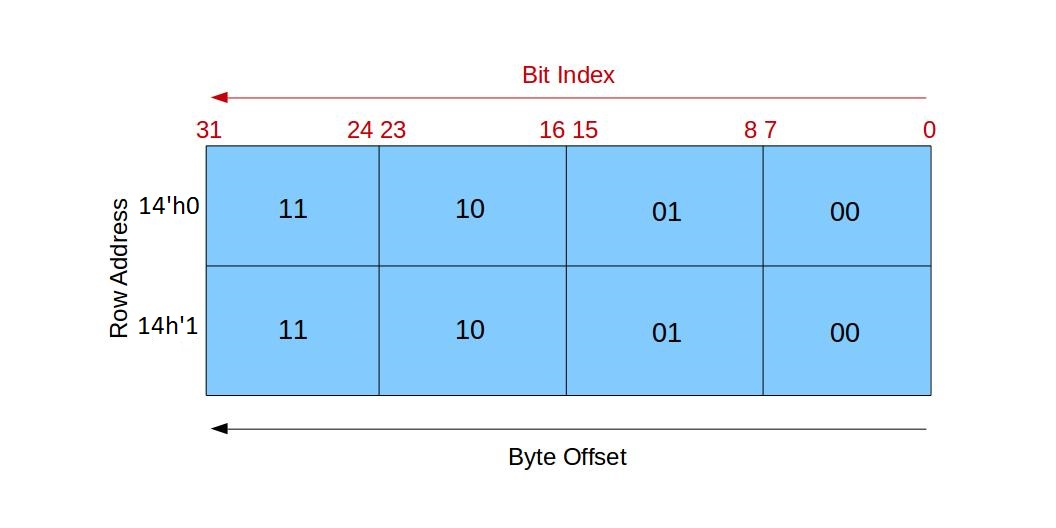
\includegraphics[width=0.8\textwidth]{figs/endianness_img.jpg}
    \caption{Block RAM organization.}
    \label{fig:endianness_img}
  \end{center}
\end{figure}

Figure \ref{fig:endianness_img} illustrates the 14-bit word addresses and the two bit byte offsets.
Observe that the RAM organization is \textbf{little-endian}, i.e. the most significant byte is at the most significant memory address (offset '11').

\subsubsection{Reading from RAMs}
Since the RAMs have 32-bit rows, you can only read data out of the RAM 32-bits at a time.
This is an issue when executing an \verb|lh| or \verb|lb| instruction, as there is no way to indicate which 8 or 16 of the 32 bits you want to read out.

Therefore, you will have to shift and mask the output of the RAM to select the appropriate portion of the 32-bits you read out.
For example, if you want to execute a \verb|lbu| on a byte address ending in \verb|2'b10|, you will only want bits \verb|[23:16]| of the 32 bits that you read out of the RAM (thus storing \verb|{24'b0, output[23:16]}| to a register).

\subsubsection{Writing to RAMs}
To take care of \verb|sb| and \verb|sh|, note that the \verb|we| input to the instruction and data memories is 4 bits wide.
These 4 bits are a byte mask telling the RAM which of the 4 bytes to actually write to.
If \verb|we|=\{4'b1111\}, then all 32 bits passed into the RAM would be written to the address given.

Here's an example of storing a single byte:
\begin{itemize}
  \item Write the byte \verb|8'ha4| to address \verb|32'h10000002| (byte offset = 2)
  \item Set \verb|we = {4'b0100}|
  \item Set \verb|din = {32'hxx_a4_xx_xx}| (\verb|x| means don't care)
\end{itemize}

\subsubsection{Unaligned Memory Accesses}
In the official RISC-V specification, unaligned loads and stores are supported.
However, in your project, you can ignore instructions that request an unaligned access.
Assume that the compiler will never generate unaligned accesses.


\subsection{Memory Architecture}
The standard RISC pipeline is usually depicted with separate instruction and data memories.
Although this is an intuitive representation, it does not let us modify the instruction memory to run new programs.
Your CPU, by the end of this checkpoint, will be able to receive compiled RISC-V binaries though the UART, store them into instruction memory, then jump to the downloaded program.
To facilitate this, we will adopt a modified memory architecture shown in Figure \ref{fig:mem_arch}.
Remember to assign their enebles properly in your logic.

\begin{figure}[hbt]
  \begin{center}
    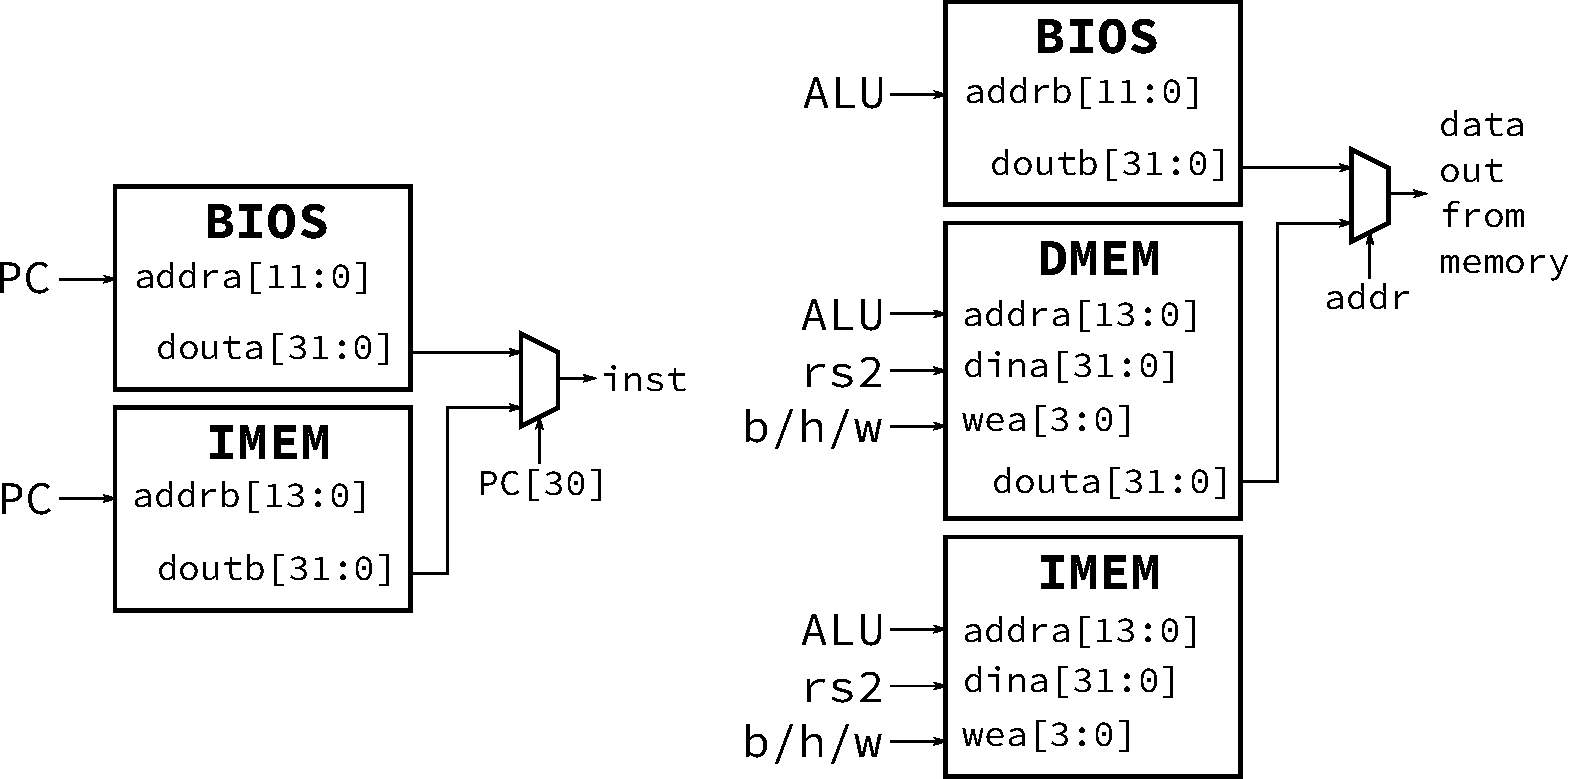
\includegraphics[width=0.8\textwidth]{figs/memory_arch.pdf}
    \caption{The Riscv151 memory architecture. There is only 1 IMEM and DMEM instance in your CPU but their ports are shown separately in this figure for clarity. The left half of the figure shows the instruction fetch logic and the right half shows the memory load/store logic.}
    \label{fig:mem_arch}
  \end{center}
\end{figure}

\subsubsection{Summary of Memory Access Patterns}
The memory architecture will consist of three RAMs (instruction, data, and BIOS).
The RAMs are memory resources (block RAMs) contained within the FPGA chip, and no external (off-chip DRAM) memory will be used for this project.

The processor will begin execution from the BIOS memory, which will be initialized with the BIOS program (in \verb|software/bios|).
The BIOS program should be able to read from the BIOS memory (to fetch static data and instructions), and read and write the instruction and data memories.
This allows the BIOS program to receive user programs over the UART from the host PC and load them into instruction memory.

You can then instruct the BIOS program to jump to an instruction memory address, which begins execution of the program that you loaded.
At any time, you can press the reset button (the right most button) on the board to return your processor to the BIOS program.

\subsubsection{Address Space Partitioning}
Your CPU will need to be able to access multiple sources for data as well as control the destination of store instructions.
In order to do this, we will partition the 32-bit address space into four regions: data memory read and writes, instruction memory writes, BIOS memory reads, and memory-mapped I/O.
This will be encoded in the top nibble (4 bits) of the memory address generated in load and store operations, as shown in Table \ref{fig:mem_space}.
In other words, the target memory/device of a load or store instruction is dependent on the address.
According to this partitioning, the reset signal should reset the PC to the value defined by the parameter \verb|RESET_PC| which is by default the base of BIOS memory (\verb|32'h40000000|).

The target memory/device is also dependent on the address type (PC or DATA).
For example the address beginning with \verb|4'h1| refers to the data memory when it is a data address, while it refers to the instruction memory when it is a program counter value.

\begin{table}[hbt]
  \begin{center}
    \caption{Memory Address Partitions}
    \label{fig:mem_space}
    \begin{tabular}{l l l l l}
      \bottomrule
      \textbf{Address[31:28]} & \textbf{Address Type} & \textbf{Device} & \textbf{Access} & \textbf{Notes} \\
      \midrule
      4'b0001 & PC   & Instruction Memory & Read-only  &\\
      4'b0100 & PC   & BIOS Memory        & Read-only  &\\
      4'b00x1 & Data & Data Memory        & Read/Write &\\
      4'b001x & Data & Instruction Memory & Write-Only & If PC[30] == 1'b1\\
      4'b0100 & Data & BIOS Memory        & Read-only  &\\
      4'b1000 & Data & I/O                & Read/Write &\\
      \bottomrule
    \end{tabular}
  \end{center}
\end{table}

Here are some examples.
When we are loading instructions, we are using a PC value as an address, and the instruction memory is read when it starts with \verb|4'h1|, while the BIOS memory is read when it starts with \verb|4'h4|.
On the other hand, when we are loading data by load instructions, the address type is Data, and the data memory is read when it starts with \verb|4'h1|, while the BIOS memory is read when it starts with \verb|4'h4|.

One tricky thing is that a store to an address beginning with \verb|4'h3| will write to both the instruction memory and the data memory, while storing to addresses beginning with \verb|4'h2| or \verb|4'h1| will write to either the instruction memory or the data memory, respectively.

\subsubsection{Memory Mapped I/O}
At this stage in the project the only way to interact with your CPU is through the UART.
The UART from Lab 5 accomplishes the low-level task of sending and receiving bits from the serial lines, but you will need a way for your CPU to send and receive bytes to and from the UART.
To accomplish this, we will use memory-mapped I/O, a technique in which registers of I/O devices are assigned memory addresses.
This enables load and store instructions to access the I/O devices as if they were memory.

To determine CPI (cycles per instruction) for a given program, the I/O memory map is also used to include instruction and cycle counters.

Table~\ref{fig:mem_map} shows the memory map for this stage of the project.

\begin{table}[hbt]
  \begin{center}
    \caption{I/O Memory Map}
    \label{fig:mem_map}
    \begin{adjustbox}{width=\columnwidth,center}
    \begin{tabular}{l l l l}
      \toprule
      \textbf{Address} & \textbf{Function} & \textbf{Access} & \textbf{Data Encoding}\\
      \midrule
      \verb|32'h80000000| & UART control & Read & \verb|{30'b0, uart_rx_data_out_valid, uart_tx_data_in_ready}| \\
      \verb|32'h80000004| & UART receiver data & Read & \verb|{24'b0, uart_rx_data_out}| \\
      \verb|32'h80000008| & UART transmitter data & Write & \verb|{24'b0, uart_tx_data_in}| \\
      \midrule
      \verb|32'h80000010| & Cycle counter & Read & Clock cycles elapsed \\
      \verb|32'h80000014| & Instruction counter & Read & Number of instructions executed \\
      \verb|32'h80000018| & Reset counters to 0 & Write & N/A \\
      \bottomrule
    \end{tabular}
    \end{adjustbox}
  \end{center}
\end{table}

You should treat I/O such as the UART just as you would treat the data memory.
The software checks the \verb|uart_rx_data_out_valid| and \verb|uart_tx_data_in_ready| signals by a load from \verb|32'h80000000|, and proceeds to a load from \verb|32'h80000004| or a store to \verb|32'h80000008| if the corresponding valid or ready signal is 1. Then your datapath will fetch \verb|uart_rx_data_out| or update \verb|uart_tx_data_in|, while asserting \verb|uart_rx_data_out_ready| or \verb|uart_tx_data_in_valid|, respectively.

The cycle counter should be incremented every cycle, and the instruction counter should be incremented for every instruction that is committed (you should not count bubbles injected into the pipeline or instructions run during a branch mispredict).
From these counts, the CPI of the processor can be determined for a given benchmark program.

\newpage
